\chapter{Authentication techiniques protocols, and architecures}

Authentication refers to the process of verifying the identity of an entity (whether it's a human, software component, or hardware element) 
before granting access to resources in a system. Authentication can be applied to various type of "actors", such as:
\begin{itemize}
    \item \textbf{Human being}
    \item \textbf{software component}
    \item \textbf{Hardware element}
\end{itemize}

\subsubsection{Authentication vs Authorization}
\begin{itemize}
    \item \textbf{Authentication (authC/authN)}: established the indetity of an entity.
    \item \textbf{Authorization (authZ)}: determines where a authenticated entity has permission to access.
\end{itemize}

\section{Authentication factors}
Authentication can be based on 3 primary factors:
\begin{itemize}
    \item \textbf{Knowledge}: Information that only the user knows and can provides as proof of ther identity.
    \item \textbf{Ownership}: Physical object or device that only the user has access to.
    \item \textbf{Inherence}: This factor relies on onique biological traits of the user (e.g fingerprint).
\end{itemize}
\textbf{N.B.} Authentication can be applied not just to human user, but also to processes and devices.

\subsection{Risks}
\begin{itemize}
    \item \textbf{Knowledge:}
    \begin{itemize}
        \item \underline{Storage} \(\rightarrow \) if passwords are stored improperly, they are vulnerable to thieft. 
        \item \underline{Demonstration} \(\rightarrow\) user might inadvertently reveal their password through social engineering.
        \item \underline{Transmission} \(\rightarrow\) if passwords are sent over ensecured channel, they can be intercepted by attackers. 
    \end{itemize}
    \item \textbf{Ownership:}
    \begin{itemize}
        \item \underline{Authentication thieft}
        \item \underline{Cloning}
        \item \underline{Unathorized usage}
    \end{itemize}
    \item \textbf{Inherence:}
    \begin{itemize}
        \item \underline{Counterfeiting} \(\rightarrow\) biometric data can be spoofed or replicated by attackers using sophisticated techiniques.
        \item \underline{Privacy} \(\rightarrow\) the use of biometric data riases the risk of biometric information being exposed.
        \item \underline{Irreversibility} \(\rightarrow\) biometric traits cannot be raplaced if compromised. 
    \end{itemize}
\end{itemize}

\section{Digital Authentication model (NIST SP800.63B)}
\begin{figure}[h]
    \centering
    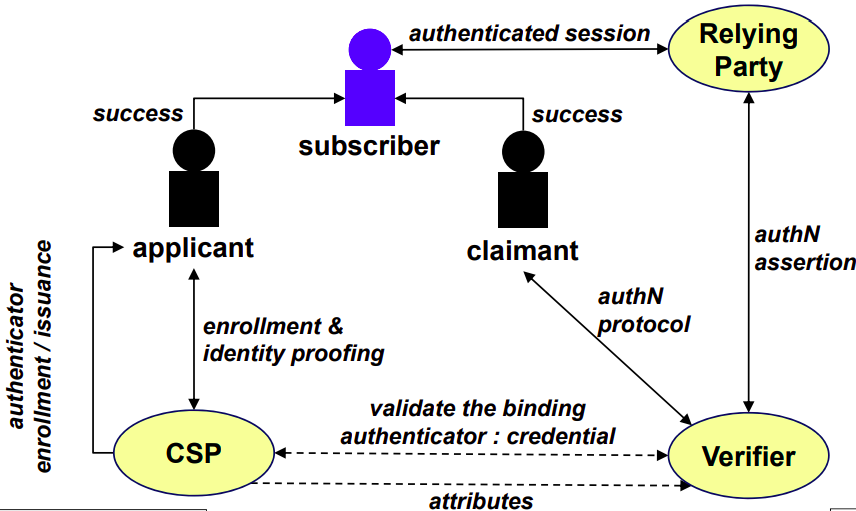
\includegraphics[width=0.5\textwidth]{/home/lorenzo/Notes/Information System Security/images/Screenshot from 2024-11-13 20-29-06.png}
\end{figure}
\textbf{Entities:}
\begin{itemize}
    \item \textbf{Subscriber}: appliacant who has succesfully completed identity proofing.
    \item \textbf{Appliacant}: an indiviual applying to established a digital identity.
    \item \textbf{Claimant}: the user trying to prove their identity to access a system or service.
    \item \textbf{Relying Party}: will request/receive an authN assertion from the verifier to asses user identity (and attributes).
    \item \textbf{Verifier}: validates the user's credential during each authentication event. 
    \item \textbf{CSP}: 
        \begin{itemize}
            \item Verifies the applicant's indetity during the initial enrollment process. 
            \item Issue a credential and bines it to an authenticator for the user.
        \end{itemize} 
\end{itemize}


\section{Generic authentication protocol}
\begin{minipage}{0.5\textwidth}
    \begin{enumerate}
        \item The user initiates an authentication request by sending their UID.
        \item The user generates a proof based on their secret, useing a secure function \(F(S_{UID})\), and send this proof to the verifier.
        \item The verifier checks if the received proof matches the stored representation of the secret.
        \item If it matches, the user is succesfully authenticated.
    \end{enumerate}
\end{minipage} 
\hspace{1cm}
\begin{minipage}{0.5\textwidth}
    \centering
    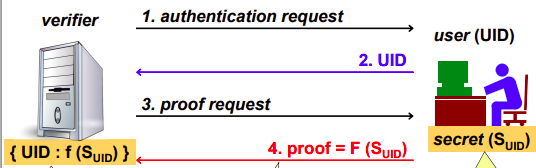
\includegraphics[width=\textwidth]{/home/lorenzo/Notes/Information System Security/images/Screenshot from 2024-11-14 11-06-55.png}
\end{minipage}



\section{Password base authentication}
\begin{minipage}{0.5\textwidth}
    \begin{enumerate}
        \item The user sends their UID and \(P_{UID}\) (= Password) to the verifier.
        \item The server verifies the proof:
        \begin{itemize}
            \item If password are stored in cleartext, it directly compares the proof with the stored password.
            \item If password are stored in hashes, it hasesh the proof and compares it to the store hash \(H_{UID}\).
        \end{itemize}
    \end{enumerate}
\end{minipage} 
\hspace{1cm}
\begin{minipage}{0.5\textwidth}
    \centering
    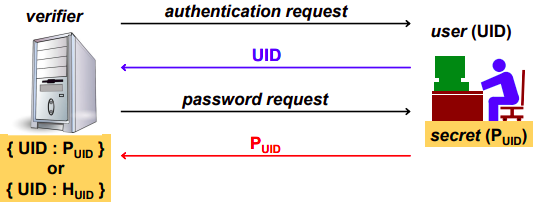
\includegraphics[width=\textwidth]{/home/lorenzo/Notes/Information System Security/images/Screenshot from 2024-11-14 11-09-10.png}
\end{minipage}

\begin{quotebox}[colframe=blue!10!white, colback=blue!5!white]{Problems of reusable Passowrds}
    \begin{itemize}
        \item \textbf{PWD Sniffing} (attackers intercept password during transmission)
        \item \textbf{PWD Database attack} (if DB contains plaintext or obfuscated PWD)
        \item \textbf{PWD Guessing} (very dangerous if it can be done offline, e.g against a list of PWD hashes)
        \item \textbf{PWD Enumeration} (PWD brute force attack)
        \begin{itemize}
            \item If PWD is limited in lenght and/or character type.
            \item If authN protocol does not block repeated failures.
        \end{itemize}
        \item \textbf{PWD Duplications} (using the same PWD for one service against another one, due to user PWD reuse)
        \item \textbf{Crypographic Aging} (as computing power grows, older crypographic methods become vulnerable to new attacks)
        \item \textbf{PWD capture via server spoofing and phishing} (attackers deceive user into givining away their PWD by pretending to be legitimate service)
    \end{itemize} 
\end{quotebox}

\begin{quotebox}[colframe=blue!10!white, colback=blue!5!white]{Password best practies}
    Suggestion to reduce password risks:
    \begin{itemize}
        \item Use alphabetical characters (upper case + lower case), digits and special characters
        \item Make passwords long (at least 8 character)
        \item Never use dictionary words
        \item Change password regularly, but not too frequently
        \item Do not reuse passwords across different services
    \end{itemize}
\end{quotebox}


\begin{quotebox}[colframe=blue!10!white, colback=blue!5!white]{Password storage}
    \begin{itemize}
        \item \textbf{Server Side:}
        \begin{itemize}
            \item Passwords should never be stored in cleartext.
            \item \underline{Encrypted passwords} aren't ideal since the server would need to know the encryption key.
            \item \underline{Better to store a password digest} (hashed password), though vulnerable to dictionary attacks.
            \item \underline{Rainbow tables} can speed up these attacks, so it’s important to add a “salt” (random variation) to each password.
        \end{itemize}
        \item \textbf{Client-side:}
        \begin{itemize}
            \item Ideally, passwords are memorized by the user, but having many passwords makes this difficult.
            \item People may resort to writing them down or using simple passwords, which is risky.
            \item \underline{Using a password manager} or encrypted file is a safer alternative.
        \end{itemize}
    \end{itemize}
\end{quotebox}


\section{The "dictionary" attack}
\begin{itemize}
    \item \textbf{Hypothesis:} The attacker knows the hash algorithm and the hashed password values.
    \item \textbf{Pre-computation:} For each word in a dictionary, compute and store its hash \(store(DB,Word,hash(World))\)
    \item \textbf{Attack process:}
    \begin{itemize}
        \item Let \(HP\) (=hash password) to be the hash of an unknown password.
        \item Lookup \(HP\) in the precomputed dictionary \((DB)\) to find a matching password.
        \item If found, output the password; if not, indicate it's "not in dictionary".
    \end{itemize}
\end{itemize}

\section{Rainbow Table attack}
Rainbow Table is a \textbf{space-time trade-off technique} that reduces storage needs for exhaustive hash tables, making certain brute-force attacks feasible within limited space.
It uses a reduction function \(r:h \rightarrow p\) (which is NOT \(h^{-1}\)) to generate chains of hashes.
\\ \textbf{Example:}
\begin{itemize}
    \item For a 12-digit password, an exhaustive hash table woudl require \(10^{12}rows(P_i:HP_i)\) 
    \item rainbow = \(10^9\) rows, each representing 1000 possible passwords.
\end{itemize}

\begin{center}
\begin{minipage}{0.5\textwidth}
    \begin{quotebox}[colframe=blue!10!white, colback=blue!5!white]{Attack}
        \centering
        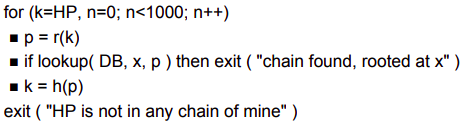
\includegraphics[width=0.8\textwidth]{/home/lorenzo/Notes/Information System Security/images/Screenshot from 2024-11-14 11-51-24.png}
\end{quotebox}
\end{minipage}
\end{center}

\section{Salting Passwords: A Defense Against Dictionary and Rainbow Table Attacks}
\textbf{Salting passwords} is a security technique used to protect stored passwords from dictionary attacks and rainbow table attacks. A salt is a unique, random string added to each password before hashing. This ensures that even if two users have the same password, their hashes will be different due to the unique salt.
\newline
\newline
\begin{minipage}[t]{0.5\textwidth}
    \subsubsection{Steps for each user (UID):}
    \begin{itemize}
        \item Generate or ask for the user's password.
        \item Create a unique, random slat for each user.
        \item Compute the salted hash:\(SHP=hash(password\ ||\ salt)\)
        \item Store the triplet \(\{UID,\ SHP,\ salt\}\)
    \end{itemize}
\end{minipage} 
\hspace{0.5cm}
\begin{minipage}[t]{0.5\textwidth}
    \subsubsection{Password Verification with Salt}
   \begin{itemize}
    \item \textbf{Claimant:} Provides their user ID (UID) and password (PWD).
    \item \textbf{verifier:} 
    \begin{itemize}
        \item Uses the UID to find the stored salted hash (SHP) and salt. 
        \item Computues \(SHP'=hash(PWD\ || \ salt)\).
    \end{itemize}
   \end{itemize}
\end{minipage}
\begin{quotebox}[colframe=blue!10!white, colback=blue!5!white]{The Linkedin attack}
In 2012, LinkedIn was breached, exposing 6.5 million unsalted SHA-1 password hashes. The lack of salting allowed attackers to crack at least 236,578 passwords through crowdsourced efforts before restrictions halted the exposure.
\end{quotebox}

\noindent\rule{1\textwidth}{0.00001pt}

\section{Strong authentication definitions}
The concept of strong authentication (authN) is crucial in ensuring secure identity verification, but it has never been formally defined with a universal definition.
Various definitions exist depending on the context, such as the European Central Bank (ECB) and PCI-DSS.

\begin{quotebox}[colframe=blue!10!white, colback=blue!5!white]{ECB definition}
    The ECB defines strong authentication as a process that involves at least two independent 
    elements from \textbf{knowledge} (e.g. password), \textbf{ownership} (e.g. smartcard), 
    and \textbf{inherence} (e.g. biometrics). The key requirement is that these elements 
    must be mutually independent, so compromising one should not affect the others. 
    Furthermore, at least one element should be \textbf{non-reusable} or \textbf{non-replicable} 
    (except for inherence), with the entire process safeguarding the confidentiality of the 
    authentication data.
\end{quotebox}

\begin{quotebox}[colframe=blue!10!white, colback=blue!5!white]{PCI-DSS Definition}
    PCI-DSS mandates \textbf{multi-factor authentication (MFA)} for access to cardholder data, 
    particularly for administrators and remote access from untrusted networks. Since version 3.2, MFA has become compulsory for remote access, 
    and the use of the same factor twice (e.g., two passwords) does not qualify as MFA.
\end{quotebox}

\section{Challenge-Response Authentication (CRA)}
Challenge-response authentication (CRA) is a widely used technique where 
a challenge is issued, and the claimant responds by solving it with a 
secret (shared or private). The challenge must be \textbf{non-repeatable} 
(usually a random nonce) to avoid replay attacks. The function used to compute 
the response must be \textbf{non-invertible}, otherwise, a listener can record the 
traffic and easily find the shared secret:
\[ if(\exists f^{-1})\ then\ K_c\ =\ f^{-1}(response, challenge)\]

\subsection{Symmetric CRA}
\begin{minipage}{0.3\textwidth}
    \vspace{-0.9cm}
    Symmetric CRA involves a shared secret (like a password or key) between 
    the claimant and verifier. This method is fast, often utilizing hash 
    functions (e.g., SHA1, SHA2, SHA3).
\end{minipage} 
\hspace{0.001cm}
\begin{minipage}{0.7\textwidth}
    \centering
    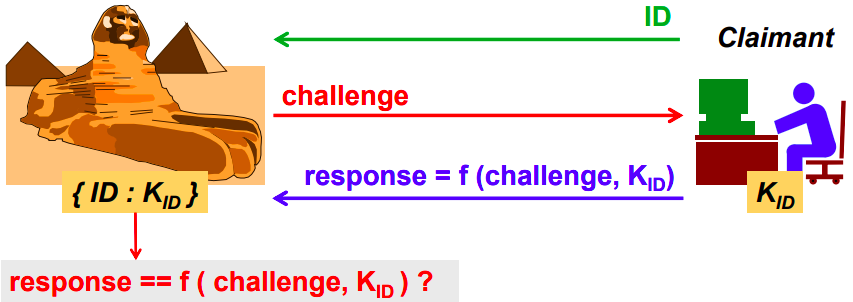
\includegraphics[width=0.7\textwidth]{/home/lorenzo/Notes/Information System Security/images/Screenshot from 2024-11-14 18-31-56.png}
\end{minipage}

\subsection{Mutual symmetric CRA}
Mutual symmetric CRA requires both parties to authenticate each other.
However, it's a old protocols so it has many vulnerabilities.

\subsubsection{Version 1: Basic Exchange}
\begin{minipage}{0.5\textwidth}
In this case, the initiator explicitly provides its claimed identity (This version is considered outdated and insecure).
\\\textbf{Process:} 
\begin{itemize}
    \item Alice sends an encrypted challenge (\(C_B\)) to Bob using the shared key \(K_{AB}\).
    \item Bob responds with an encrypted challenge (\(C_A\)) for Alice, also using \(K_{AB}\).
\end{itemize}
\end{minipage} 
\hspace{0cm}
\begin{minipage}{0.5\textwidth}
    \centering
    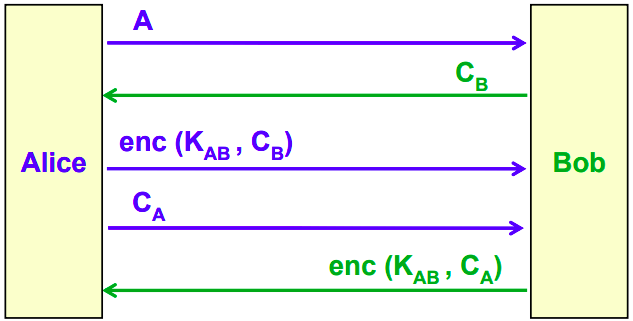
\includegraphics[width=0.7\textwidth]{/home/lorenzo/Notes/Information System Security/images/Screenshot from 2024-11-15 11-52-51.png}
\end{minipage}

\subsubsection{Version 2: Improved Performance}
\begin{minipage}{0.5\textwidth}
    Optimized by reducing the number of messages, which improves performance without compromising security.
    \\ \textbf{Process:}
    \begin{itemize}
        \item Alice includes her identity \((C_A)\) and sends an encrypted challenge (\(C_B)\) in the same message.
        \item Bob responds with his encrypted challenge \(C_A\)to complete the exchange.
    \end{itemize} 

\end{minipage} 
\hspace{0cm}
\begin{minipage}{0.5\textwidth}
    \centering
    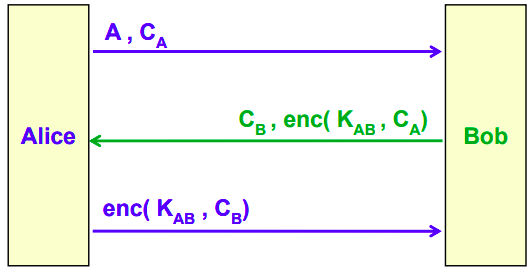
\includegraphics[width=0.7\textwidth]{/home/lorenzo/Notes/Information System Security/images/Screenshot from 2024-11-15 12-04-56.png}
\end{minipage}

%Now I give you some text and I want that you resume it. I don't want many list (this it no means that I don't want there to be any) I want also that you riorganized the sections 
\begin{quotebox}[colframe=blue!10!white, colback=blue!5!white]{Attack on Mutual Symmetric CRA}
    \begin{minipage}{0.5\textwidth}
        \vspace{-0.5cm}
        A potential attacker, "Mike" (posing as Alice), exploits the protocol by mimicking responses:
        \begin{itemize}
            \item The attacker intercepts Alice's identity \((C_A)\) and Bob's challenge \((C_B)\).
            \item The attacker uses the shared key \(K_{AB}\) to manipulate responses and mimic both parties.
        \end{itemize}
    \end{minipage} 
    \hspace{1cm}
    \begin{minipage}{0.3\textwidth}
        \centering
        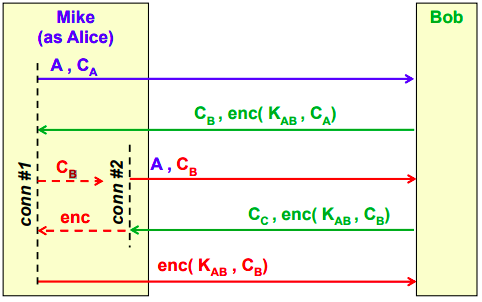
\includegraphics[width=\textwidth]{/home/lorenzo/Notes/Information System Security/images/Screenshot from 2024-11-15 12-09-09.png}
    \end{minipage}
\end{quotebox}

\subsection{Asymmetric CRA}
\begin{minipage}{0.6\textwidth}
%	\vspace{-0.5cm}
    \textbf{Process:}
    \begin{itemize}
        \item A \textbf{random nonce (R)} is generated by the Verifier.
        \item The verifier encrypts \(R\) using the user's public key (\(ID.PK\)) and sends it to the Claimant:
        \(C=enc(ID.PK,R)\)
        \item The Claimant decrypts \(C\) using their private key (\(ID.SK\)) and sends \(R\) back in cleartext:
        \(response=dec(ID.SK,C)\)
        \item The Verifier validates: \(valid(ID)\ \&\&\ (response\ ==\ R)\).
    \end{itemize}
\end{minipage} 
\hspace{0.2cm}
\begin{minipage}{0.4\textwidth}
    \centering
    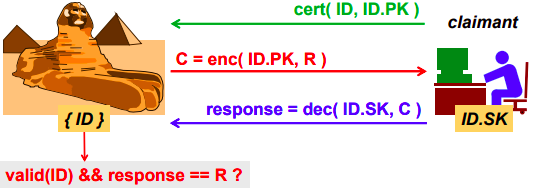
\includegraphics[width=\textwidth]{/home/lorenzo/Notes/Information System Security/images/Screenshot from 2024-11-15 12-43-33.png}
\end{minipage}
\subsubsection{Applications}
\begin{itemize}
    \item  Widely implemented in secure communication protocols like IPsec, SSH, and TLS.
    \item Fundamental in modern authentication frameworks such as FIDO.
\end{itemize}
\begin{quotebox}[colframe=blue!10!white, colback=blue!5!white]{Asymmetric CRA analysis}
    \begin{minipage}{0.5\textwidth}
        \vspace{-1.1cm}
        \subsubsection{Security:}
        \begin{itemize}
            \item It's the strongest mechanism.
            \item Does not require the Verifier to store any shared secret, reducing potential attack vectors.
        \end{itemize}
     \end{minipage} 
     \hspace{0cm}
     \begin{minipage}{0.5\textwidth}
        \subsubsection{Problems:}
        \begin{itemize}
            \item It \textbf{slower} compared to symmetric methods.
            \item If designed inaccurately may lead to an involuntary signature
            by the Claimant.
            \item Trust issues managing root certificates, name constraint, and certificate revocation.
        \end{itemize}
     \end{minipage}
\end{quotebox}

\section{One-Time Password(OTP)}
\begin{minipage}{0.5\textwidth}
%	\vspace{-0.5cm}
One-Time Passwords are temporary and valid for a single use in an authentication session. They mitigate risks like password reuse and passive sniffing but can still be vulnerable to man-in-the-middle (MITM) attacks. 
\end{minipage} 
\hspace{1cm}
\begin{minipage}{0.5\textwidth}
    \centering
    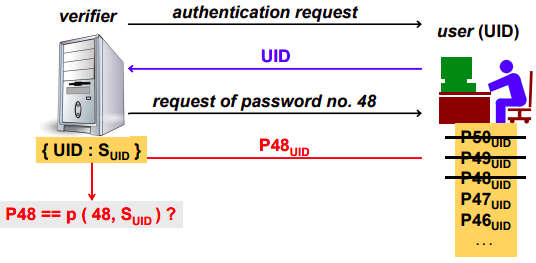
\includegraphics[width=0.7\textwidth]{/home/lorenzo/Notes/Information System Security/images/Screenshot from 2024-11-15 13-11-17.png}
\end{minipage}